\documentclass{standalone}
\begin{document}
The origin of quantum computation is typically attributed to Richard Feynman, in a keynote address at the 1981 `First Conference on the Physics of Computation' at MIT~\cite{Feynman1982}. Feynman's speech discussed the problems of simulating physical systems computationally. As one candidate solution, he proposed the technique of quantum simulation: using the controlled dynamics of one quantum system to probe the dynamics of another. 
\par
At the same conference, Peter Benioff presented a paper on using Hamiltonian evolution of a spin-lattice system to realise a Turing Machine~\cite{Benioff1986}, an abstract model used to study universal classical computation. The state of the system is represented by an `tape', broken into cells which store binary values. The computation is carried out by a `head' or processor, which can read and write bits and move along the tape according to a programme~\cite{Deutsch1985}. This simplified model is often employed in complexity theory, where the number of `steps' taken by the head and number of cells used give the temporal and spatial resources consumed in the computation.  In essence, Benioff proposed a quantum implementation of classical computation, encoding the binary state in the spin of the lattice, where the reading and writing would be controlled by spin-spin interactions~\cite{Benioff1986}.\\
Feynman's proposed quantum simulator followed a similar scheme, premised on applying annihilation, creation and `number' operators to different components of the system. This is analogous to subtracting, adding or reading a value on a Turing machine tape. Feynman similarly noted that a two-level spin system would serve as the smallest implementation of such a device~\cite{Feynman1982}.
\par
Both schemes are early proposal of the `qubit', a two-level quantum system used as a building block in computation and communication protocols. The earliest example is attributed to Stephen Wiesner, who discussed using polarisation states of photons to implement a secure serial number in a `Quantum Money' scheme~\cite{Wiesner1983}. Wiesner developed this scheme in the 70s, but was unable to publish the work until after Feynman and Benioff's talks~\cite{Brassard2006}. The term qubit was later coined by Schumacher, in his paper on a quantum analogue of Shannon's noiseless coding theorem~\cite{Schumacher1995a}.
\par
The `quantum advantage' in these early proposals is presented somewhat abstractly. In Benioff's paper, he argues that implementing computation directly on a physical system should offer speed, size and energy advantages over existing classical implementations~\cite{Benioff1986}, but doesn't discuss these effects as originating from the quantum mechanical nature of the system. In Feynman's talk, however, the advantages of using a quantum simulator are summarised succinctly in the popular quote:\\
\textquote{Nature isn't classical, dammit, and if you want to make a simulation of nature you better make it quantum mechanical!}

\section{Quantum Turing Machines}\label{sec:QTM}
This question of what computational resources we need to simulate arbitrary physical systems was formalised by Deutsch in his 1985 paper `Quantum theory, the Church-Turing principle, and the universal quantum computer'. This paper is widely considered as establishing the theory of quantum computation, as it formally defines the principle of `universal quantum computing'~\cite{Deutsch1985}. 
\par
In this paper, Deutsch relates the Church-Turing thesis, a statement about the nature of computationally solvable problems, to the problem of simulating physical systems highlighted by Feynman. This gives a novel definition of a universal computing machine: any device capable of perfectly simulating a finitely realisable physical system with finite resources~\cite{Deutsch1985}. \\
The classical Turing Machine fails this definition, as binary numeral systems cannot be used to represent continuous real numbers, as would be required to simulate classical physical systems~\cite{Deutsch1985}. Jozsa describes this strengthened Church-Turing-Deutsch thesis as requiring that questions of `What is computable?'\ be grounded in the laws of physics and not characterised by mathematics alone~\cite{Jozsa1997}.
\par
Instead, Deutsch introduces a model of a quantum Turing machine, which passes this Church-Turing-Deutsch criterion for simulating finite quantum mechanical systems. This is an extension of Feynman's ideas, and a quantum measurement automaton discussed by Albert~\cite{Albert1983}. Unlike Benioff's proposal, which restricted the system to classical computational states, the state of this device is explicitly quantum mechanical, allowing any state in the Hilbert space $\mathcal{H}=\mathbb{C}^{2^{n}} \otimes \mathbb{C}^{2^{m}}$ defined by the $n$ qubits in the processor $m$ qubits in the `tape'. The evolution of the combined processor-tape system is the described with unitary dynamics~\cite{Deutsch1985}. \\
Interestingly, Deutsch proves that a quantum Turing machine would still be restricted to solving the class of `General Recursive' functions defined as computable under the Church-Turing thesis~\cite{Deutsch1985}. However, he goes on to demonstrate that even with this restriction, such a quantum Turing machine would be capable of simulating classical computation, and of simulating a much broader class of physical systems than a classical device~\cite{Deutsch1985}.
\par
In this paper, Deutsch also set out an algorithm which demonstrates the ability of a quantum computer to perform tasks faster than any classical device. In particular, he constructs a problem where we are given access to an `oracle', which evaluates a function $f:\mathbb{F}_{2}^{2}\rightarrow\{0,1\}$ and returns the result, where $\mathbb{F}_{2}^{n}$ is the space of $n$-bit binary strings.\\
We are tasked with determining if the function is equal for all inputs (`constant'), or if it returns $0$ for half of the inputs and $1$ for the other (`balanced'), in as few evaluations or `orcale queries' as possible. An extension of this problem to n-bit functions $f:\mathbb{Z}_{2}^{n}\rightarrow\mathbb{Z}_{2}$, called the Deutsch-Jozsa algorithm, was proposed in 1992, and more dramatically illustrates the computational advantage of the quantum Turing machine~\cite{Deutsch92}.
\par
To answer this question deterministically, a classical computer would need to evaluate $f$ for $\frac{2^{n}}{2}+1$ inputs, half of the possible set. However, it can be shown that by preparing a quantum computer in a superposition of all $n$-bit binary strings $\ket{\psi}=\frac{1}{\sqrt{2}^{n}}\sum_{x\in\mathbb{F}_{2}^{n}}\ket{x}$, it suffices to evaluate $f$ once. Deutsch dubbed this behaviour `quantum parallelism', as it relies both on the ability of quantum states to exist in superposition, and for the existence of relative phase between states such that interference between then results in a deterministic answer.
\par
\pagebreak
\section{The Nature of Quantum Speedup}\label{sec:WhatSpeedup}
The Deutsch-Jozsa algorithm demonstrates a dramatic reduction in query complexity, but this is relative to a classical algorithm sequentially testing inputs to be able to give a deterministic answer. In reality, a classical computer testing random inputs would be able to answer the Deutsch-Jozsa problem with a certain probability in much less than $\frac{2^{n}}{2}$ trials. \\
In classical computational complexity theory, problems of this type belong to a class called `Bounded-error Probability Polynomial' ($\BPP$); the class of problems where an efficient algorithm\footnote{`Efficient' problems are generally defined as those with a running time polynomial in the problem size. These are the classes $\P$ (deterministic Polynomial), and $\BPP$ for classical computing, and $\BQP$ for quantum computing.} including a randomised process can return the correct answer with an error that is bounded by a constant, independent of the problem size~\cite{Bennett1997}. The quantum analogue of this class, Bounded-error Quantum Polynomial ($\BQP$), is considered the class of problems efficiently solvable on a quantum computer~\cite{Bernstein1997}.
\par
The term `polynomial' in the above definitions refers to the `time' taken to complete the computation, as a function of the number of bits in the problem $n$. In the Turing machine picture, this is the number of steps in the computation, but it can equivalently be defined as the number of logic gates acting on $n$ binary bits in a boolean circuit. In 1993, Yao demonstrated that an equivalent `circuit' model exists for quantum computing, and that any quantum circuit is capable of simulating a quantum Turing machine~\cite{Yao1993}. This circuit model, where elementary unitary matrices are acted in succession on $n$-qubits to implement a computation $U$, is the framework used to develop and analyse quantum algorithms. \\
The use of query complexity might seem to be `hiding' the true computational complexity of the problem: what if the oracle requires a long time to evaluate? However, in this and other problems the oracle is evaluating a classical boolean function $f$, which thus has an efficient implementation as as quantum circuit~\cite{Bernstein1997}. 
\par
Following the work of Deutsch and Jozsa, the question of quantum speedup became: do there exist problems which are efficient for a quantum computer to solve, but which are `harder' than $\BPP$ for a classical device?

\subsection{Beating BPP}\label{sec:exponentialspeedup}
This question was answered in a series of three papers in 1997, which first established the existence of, and then developed explicit quantum algorithms for, problems in $\BQP$ which for a classical computer require a computational time that scales exponentially in the size of the problem~\cite{Bennett1997}. 
\par
The existence of this exponential quantum speedup over classical computation was first proved by Bernstein and Vazirani in their paper on quantum computational complexity theory~\cite{Bernstein1997}. As well as demonstrating the possibility of exponential speedup, this paper formalised Deutsch's quantum Turing machine construction, and used it to prove a number of properties about $\BQP$, In particular, they demonstrated that $\BPP\subseteq\BQP$; that a quantum computer is capable of efficiently simulating efficient classical algorithms, including those assisted by random number generation.
\par
The first explicit construction of such a problem was given by Simon in 1994, again using an `oracle' formulation of the computation~\cite{Division1998a}. In Simon's problem, the oracle implements a binary function $f: \mathbb{F}_{2}^{n}\rightarrow\mathbb{F}_{2}^{n}$, such that for two binary strings $x,y\in\mathbb{F}_{2}^{n},\;f(x)=f(y)\Leftrightarrow x = y \oplus s$, for some constant string $s$. We are tasked with finding the string $s$ in as few queries as possible. For a quantum computer, this algorithm requires only $O(n)$ oracle queries. In contrast, a classical method would require $O\left(2^{\frac{n}{2}}\right)$~\cite{Division1998a}.\\
Simon's algorithm is another example of a `toy' problem, but the techniques presented were then applied by Peter Shor to develop a general quantum algorithm capable of solving two mathematical problems: Prime Factorisation and the Discrete Logarithm~\cite{Division1998a,Shor1997}. In complexity theoretic terms, they belong to the class $\NP$, problems which require an exponential amount of time to solve, but for which a proposed solution can be checked efficiently~\cite{Bennett1997}.
\par
It is believed that a polynomial-time classical algorithm for both problems does not exist. In face, the presumed computational hardness of prime factorisation is what guarantees the security of RSA and other cryptographic protocols currently relied upon for secure encryption~\cite{Nielsen2000}. The discovery of an efficient quantum algorithm spurred a great deal of interest in quantum computing, as it raised the possibility of devices capable of breaking most if not all of modern cryptography~\cite{Shor1997}. 
\par
The existence of problems that reside in the class $\BQP$ but for which no efficient classical algorithm exists, further clarifies the idea of Feynman and Deutsch that a classical computer cannot efficiently simulate a quantum system. Any efficient simulation of arbitrary quantum systems would be also be able to implement quantum computations, and would in turn give us efficient classical algorithms for problems like prime factorisation~\cite{Shor1997}.

\subsection{NP-Complete Problems}\label{sec:notNP}
While prime factorisation and the discrete logarithm are difficult to solve classically, they do not belong to the so called $\NP$-complete problems; problems in the class $\NP$ for which \emph{any other} problem in $\NP$ can be encoded as an instance of the problem~\cite{ComplexityZoo}. As a result of this `completeness' property, the $\NP$-complete problems are considered some of the most import in computer science~\cite{Bennett1997}.
\par
In 1996, Lov Grover developed a quantum algorithm capable of solving arbitrary $\NP$ problems, including the $\NP$-complete problems, using the polynomial `verifier' of a candidate solution implemented as an oracle~\cite{Grover1996}. This algorithm is commonly referred to as `quantum search', as it was developed as a technique for searching for a single item in a set of $N=2^{n}$ entries. A classical, brute-force search would, in the worst case, require testing all $N$ items, an in general requires testing $O(N)$. \\
Grover's quantum algorithm, however, can succeed in $O(\sqrt{N})$ trials, a more modest quadratic reduction in the oracle complexity. The techniques employed are very similar to the Deutsch-Jozsa algorithm, applying the oracle to a uniform superposition of $N$ inputs to `mark' the solution. This is followed by the application of a `diffusion' operator, which boosts the amplitude of the marked state. THis pair of operations is called the `Grover step', and the amplitude of the state corresponding to the solution is maximal after $O(\sqrt{N})$ such steps~\cite{Grover1996}.\\
However, such a brute-force search is likely not optimal for realistic database searching. For example, if the data can be sorted based on a certain criteria, then a `bracketing and bisection' technique based on testing random entries in the sequence can succeed in $O(\log_{2}(N))$ trials. However, this kind of brute force problem does arise when considering $\NP$-complete problems, such as optimisation problems. Classical algorithms for such problems often use heuristics to try and aid the search through the space of possible solutions.\\
In this case, Grover's algorithm allows a quantum computer to achieve a quadratic speedup for any $\NP$-complete problem. Shortly afterwards, it was shown by Bennett et al.\ that Grover's quadratic speedup is likely optimal for any quantum algorithm tackling $\NP$-complete problems~\cite{Bennett1997}.
\par
These results have demonstrated the nature of quantum speedup. Quantum computing seems provably stronger than classical computation when it comes to simulation of physical systems, as it satisfies the Church-Turing-Deutsch thesis. A quantum computer can simulate classical algorithms, as $\BPP\subseteq\BQP$. It has also been proven that there exist problems believed to be in $\NP$, which reside in $\BQP$ for a quantum computer. However, it is believed that quantum computers cannot offer a greater than quadratic speedup for the $\NP$-complete problems. 

\section{What is the Origin of Quantum Speedup?}
Given the existence of quantum speedup, it is interesting to ask what aspects of quantum mechanics underlie this effect. This is not only an interesting theoretical question, but also relevant to our attempts to realise quantum technologies. Control of quantum systems, including isolating them from the effects of decoherence, represents a significant challenge~\cite{Shor1997}. Understanding the origin of quantum speedup thus helps us to understand what criteria our experimental devices will need to satisfy.
\par
In section~\ref{sec:QTM}, we introduced the notion of `quantum parallelism', the ability of a quantum system to exist in superpositions of multiple states and an oracle function to be evaluated simultaneously across all inputs. Holevo's bound tells us, however, that while it is possible for the system to be in a superposition of $2^{n}$ states, we can only access classical information of $1$ of these states at a time~\cite{holevo1973}. As such, we also require interference effects to be present in the computation, such that the system converges to a solution.\\
However, in a 1997 paper, Jozsa discusses the fact that superposition and interference are both effects demonstrated by classical waves~\cite{Jozsa1997}. Instead, Jozsa argues that the critical feature of quantum mechanics is the existence of entangled states. 

\subsection{Entanglement and Quantum Computing}\label{sec:entanglement}
A general quantum state on $n$-qubits, $\ket{\psi}$, exists in the Hilbert space $\mathcal{H}_{2^{n}}$. If this state can be decomposed into a tensor product of states on smaller Hilbert spaces, then it is called a `separable' or `product' state. If no such decomposition exists, the state is said to be entangled~\cite{Nielsen2000}. This definition is exact for pure states, though entanglement for mixed states is much less well characterised~\cite{Laflamme2001}. 
\par
In his paper, Jozsa considers the example of a classical system with $2^{n}$ states, constructed out of $n$ strings each in a superposition of their two lowest-energy vibrational modes. However, composite classical systems combine under the Cartesian product~\cite{Jozsa1997}
\begin{equation}
    A\times B = \{(a,b) : a\in A, b\in B\} \implies \left| A\times B\right| = \left|A\right| + \left|B\right|
\end{equation}
 in contrast to quantum systems which use the tensor product~\cite{Nielsen2000}
\begin{equation}
    A\otimes B = \{(ab) : a\in A, b\in B\} \implies \left|A\otimes B\right| = \left|A\right|\cdot\left|B\right|.
\end{equation}
As a result, this physical system remains a separable product of $n$ individual subsystems. The phenomenon of entanglement, where a physical system cannot be described as a combination of smaller subsystems, is not possible classically~\cite{Jozsa1997}. \\
This argument was extended in a later paper in collaboration with Ekert~\cite{Ekert1998}. In this paper, they also consider the possibility of constructing a classical simulator based on a superposition of $2^{n}$ vibrational modes, which would exploit an isomorphism between $\otimes^{n}\mathcal{H}_{2}$, the Hilbert space n qubits, and $\mathcal{H}_{2^{n}}$, the Hilbert space of one, $2^{n}$-level quantum system. In this picture, the `isomorphism' would allow us to label certain states of the classical simulator as entangled~\cite{Ekert1998}. \\
However, the authors demonstrate that such a classical simulator cannot be implemented without an exponential overhead in some physical resource, and thus cannot be considered realistic. For example, a system of $n$-qubits, each with the same `energy gap', would require an amount of energy to control that grows linearly in $n$. However, for the $2^{n}$ level classical simulator, the number of energy levels and thus the energy required to implement it grows exponentially in $n$~\cite{Ekert1998}.\\
A similar argument applies if we instead consider a different classical simulator where the $2^{n}$ levels accumulate below a finite upper bound~\cite{Jozsa2003}. In this case, the precision required to resolve these levels grows exponentially in $n$ and the simulator is not physically feasible. Thus, the authors argue, the phenomenon of quantum speedup is due precisely due to the existence of entangled states.  
\par
Jozsa and Ekert also indicate the presence of entanglement in existing descriptions of quantum algorithms. For example, when an oracle gate, $O_{f}$, is applied to a superposition of input strings $\frac{1}{2^{n}}\sum_{x\in\mathbb{F}_{2}^{n}}\ket{x}$, the resulting state is an entangled state of each input with its evaluation $\sum_{x\in\mathbb{F}_{2}^{n}}\ket{x}\ket{f(x)}$~\cite{Jozsa1997}. Ekert and Jozsa also demonstrate the existence of entanglement in the quantum Fourier transform, a subroutine employed in Simon's and Shor's algorithms~\cite{Ekert1998}.

\subsubsection*{Impact on Experimental Efforts}
This identification of entanglement as a the key resource for quantum speedup had a significant impact on the quantum computing community. In particular, it called into question a series of early quantum computing experiments realised using NMR systems~\cite{Braunstein1999,Linden2001} It was shown by Braunstein et al.\ that, for sufficiently high levels of noise, the `pseudo-pure' states used in NMR computing would remain separable throughout the computation~\cite{Braunstein1999}. \\
This analysis in fact demonstrated that all previous NMR experiments had systematic noise above this threshold. A subsequent paper by Linden and Popsecu explicitly demonstrated that executions of Shor's algorithm requires the system to become entangled, again ruling out previous NMR results~\cite{Linden2001}. A similar result was also shown for Grover's algorithm~\cite{Braunstein2001}.\\
This demonstrates the ability of theoretical studies into the foundations of quantum theory to influence the course of quantum technologies.

\subsection{Is Entanglement Necessary?}\label{sec:classicalsim}
When trying to understand quantum speedup, it can also be instructive to consider the classical information required to fully describe a quantum system. Any quantum dynamics which can be efficiently simulated classically cannot, by definition, realise quantum speedup. The inverse statement, that a lack of efficient classical simulation implies quantum speedup, is not necessarily true, as it assumes no better classical simulation method exists. Nonetheless, an exponential classical complexity is considered indicative of quantum advantage~\cite{Jozsa2003}.
\par
If we consider the classical information required to fully characterise a quantum state, then a product state of $n$ qubits $\ket{\psi}=\bigotimes_{i=1}^{j}\ket{\phi}_{j}$, can be completely described with $O(j)$ complex numbers~\cite{Jozsa1997}. In contrast, entangled states requires $O(2^{n})$ numbers to describe the system completely~\cite{Jozsa1997}. \\
This exponential classical description as a result of entanglement can also be applied to descriptions of quantum circuits. A given computation on $n$ qubits involves a $2^{n}\times2^{n}$ unitary matrix $U$. However, by decomposing this unitary into a sequence of elementary gates acting on one or two qubits, we can reduce this complexity to $O(\poly(n))$~\cite{Ekert1998}. The overall complexity of the computation is then polynomial in $n$ if the state can be described as a product state at all steps~\cite{Ekert1998} 
\par
Jozsa \& Linden used this observation to give a slightly more restricted definition of entanglement as a resource for quantum computation~\cite{Jozsa2003}. In particular, it is not sufficient for only a small, bounded subset of the qubits to become entangled. The authors define the notion of a `p-blocked state', which can be split into subsystems of at most $p$ qubits, and show that a quantum computation is efficiently simulable if at all steps there exists such a decomposition~\cite{Jozsa2003}. Instead, the entanglement in the system must be unbounded, growing to include all qubits present in the computation. They then explicitly demonstrate that, for Shor's algorithm, the entanglement grows in precisely this unbounded way~\cite{Jozsa2003}.

\subsubsection{Efficient Simulation of Entangled States}\label{sec:gk}
Interestingly, they authors also show that we can approximately simulate our quantum computation to within an error $\eta$, provided there exists at all steps a $p$-blocked state $\epsilon$-close to the `true' state of the computation where $\epsilon=c^{T}\eta$, $T$ is the number of steps in the circuit, and $c$ is a constant less than one~\cite{Jozsa2003}. \\
This pair of results significantly constrain the quantum advantage offered by entanglement alone. A similar result was found by Vidal, who developed a novel method for simulating 1D-spin chains with `restricted' entanglement. In particular, he showed that if the entanglement measure $E_{\chi}\equiv\log_{2}(\chi)$, where $\chi$ is the Schmidt-Rank of the state, grows only logarithmically in the system size, then it admits an efficient classical decomposition~\cite{Vidal2003}.
\par
Jozsa \& Ekert's conclusions about entanglement were challenged by Laflamme et al., in response to Braunstein's argument against NMR quantum computing on the grounds of separability~\cite{Laflamme2001}. Laflamme argued that, whereas the non-local behaviour of entangled systems gives a clear advantage in quantum communication protocols, the significance of entanglement to quantum computing is much less clear. In particular, they argued that the apparent significance of entanglement could be explained by the computational description employed by Jozsa and Ekert, in terms of the $2^{n}$ complex amplitudes of the $n$-qubit state~\cite{Laflamme2001}.\\
As a counter example, Laflamme cites the `Heisenberg picture' of quantum computation developed by Gottesman \& Knill. The Heisenberg picture is a construction of quantum mechanics where time-evolution is carried by the operators rather than by the quantum states~\cite{Nielsen2000}. The Gottesman \& Knill construction similarly allows the quantum circuits acting on a special subset of quantum states to be described in terms of their effect on groups of Pauli operators alone~\cite{Gottesman1999a}. 
\par
Originally developed in the context of quantum error correction codes, Gottesman's formalism is predicated around groups of operators $\mathcal{S}\subseteq\mathcal{P}_{n}$, subgroups of the $n$-qubit Pauli group. Gottesman showed that there exists subgroups on $n$ qubits $\mathcal{S}:\vert\mathcal{S}\vert=2^{n}$, which have a unique +1 eigenstate $\ket{\phi}:s\ket{\phi}=\ket{\phi}\forall s\in\mathcal{S}$. These eigenstates are called `stabilizer' states, as they are stabilised by the group $\mathcal{S}$.\\
The action of these stabilizer groups can be entirely described by its generating set, a subset of independent elements which can be multiplied together to produce all other elements in the group. Because the stabilizer operators have a common eigenstate, the group is abelian, meaning it's $2^{n}$ elements can be described using just $n$ generators. The action of a unitary $U$ acting on a stabilizer state can then be described by evolving the stabilizer generators $s_{i}:i\in\{1,\cdots, n\}$ under the relation $s_{i}' = UsU^{\dagger}$. \\
This allows the stabilizer states to be fully characterised using $n$ sets of $n$ Pauli operators. Examples of stabilizer states include the computational basis states, but it also includes a number of entangled states. For example, the maximally entangled Bell state $\ket{\Psi}_{+}=\frac{1}{\sqrt{2}}(\ket{01}+\ket{10})$, is stabilised by the generators $X\otimes \mathbb{I}$ and $\mathbb{I}\otimes X$. Interestingly, this state demonstrates `unbounded' two-qubit entanglement.
\par
For a general computation $U$, these stabilizer generators are $2^{n}\times2^{n}$ matrices, so this description remains classically complex. However, for a large number of elementary quantum gates, including the `entangling' CNOT gate, their action on the stabilizer states can be efficiently computed classically~\cite{Gottesman1999a}.\\
These operations are commonly referred to as the Clifford group, defined as the matrices~\cite{Gottesman1999a}
\begin{equation}\label{eq:Clifford}
U:UPU^{\dagger}\in\mathcal{P}_{n}\;\forall P\in\mathcal{P}_{n}.
\end{equation}
As they only map Pauli operators to other Pauli operators, their action on the stabilizer states is simply given by appropriately updating the Pauli operators that generate each group. \\
While this is a restricted set of operations and states, the stabilizer formalism is nonetheless capable of describing entangled states. It can also be used to simulate intrinsically `quantum' protocols, such as quantum teleportation, efficiently~\cite{Aaronson2004a}.
\par
Laflamme thus argued that apparent requirement of entanglement for quantum speedup could be perhaps understood as a consequence of the amplitude formalism that Jozsa, Ekert, Linden and Popescu used to describe quantum states and their simulation~\cite{Laflamme2001}. Instead, given the efficient simulability of Clifford circuits, and that mixed-state entanglement is not well understood, Laflamme proposed that it is the full unitary dynamics that gives a quantum computer its advantage~\cite{Laflamme2001}.
\par
Jozsa \& Linden acknowledge Laflamme's argument in the conclusion to their paper, agreeing that this apparent requirement for unbounded entanglement derives from their chosen classical description of the quantum states, and that different descriptions of quantum mechanics would have different sets of efficiently-described states. 
\par
The debate over the role of entanglement in computation continues today. For example, a recent result that could be seen as both supporting Laflamme's \& Jozsa's arguments is the demonstration by Van den Nest of universal quantum computation based only on states with a small amount of entanglement under the `Entanglement Entropy' measure~\cite{VanDenNest2013}. Interestingly, even with access to this limited amount of entanglement, he demonstrated that these states can realise arbitrary unitary dynamics, and such be used to realise universal quantum computation. This could be interpreted as demonstrating the power of entanglement alone, or the role of unitary dynamics.
\par
This debate illustrates the difficulty of demonstrating the origins of quantum advantage; the absence of an efficient classical description is not a clear indicator of quantum speedup, as this description depends on the formalism chosen. For each description $\mathcal{D}$, there exists a corresponding property $\text{prop}\left(\mathcal{D}\right)$ that is required for quantum speedup~\cite{Jozsa2003}. In some sense, we can argue that a system demonstrating quantum speedup must satisfy $\text{prop}(\mathcal{D})\;\forall\;\mathcal{D}$~\cite{Jozsa2003,Laflamme2001}. However, the existence of an efficient classical method is a clear signifier of the absence of quantum advantage, and so classical simulations of quantum computation are still an effective way to study the `power' of a quantum computation.
\par
\section{Fault Tolerant Quantum Computing}\label{sec:FTQC}
Despite continued improvements in qubit control, quantum computation still has to contend with the effects of decoherence and environmental noise~\cite{Nielsen2000}. This has lead to the notion of fault tolerant schemes, designed to protect the quantum information throughout the computation~\cite{Nielsen2000}. 
\par
In a fault tolerant quantum computer, the information is encoded in multiple physical qubits using a quantum error correction code. These codes can also be described using Gottesman's stabilizer formalism; the $2^{m}$ basis states of the codespace are the $+1$ eigenstates of a stabilizer group with $k=n-m$ generators, acting on $n$ qubits. The computation is then performed using `logical' gates that act on the encoded states~\cite{Gottesman1997}.\\
If an error occurs on one of the physical bits during a logical gate, it can be detected by a $-1$ outcome when measuring the stabilizer generators~\cite{Gottesman1997}. By measuring the generators at each step in the computation, we can identify and correct any errors that occur~\cite{Nielsen2000}.\\
However, this also requires that we construct our `logical' gates in a fault tolerant way. If the logical gates induce multiple errors on each encoded qubit, then we are no longer able to deterministically detect and correct them~\cite{Gottesman2009}. Instead, we typically require that our logical gates be `transversal': that they require no multi-qubit gates within a single code block. This prevents an error on one physical bit from spreading to other qubits, reducing the probability of our code failing~\cite{Nielsen2000,Gottesman2009}.
\par
Unfortunately, it is known that no stabilizer error-correction code can have a set of transversal gates that is also universal for quantum computation~\cite{Eastin2009}. In fact, most stabilizer codes admit only Clifford group operations as their transversal gate set. As the states of the code are entirely characterised by a stabilizer code, this means that not only are these codes not-universal, but their action can be efficiently simulated classically. It was in fact shown by Aaronson \& Gottesman that these Clifford circuits are strictly \emph{weaker} than a classical computer~\cite{Aaronson2004a}. We thus need some way to boost our Clifford circuits to universality, and to do so in a fault tolerant way. 
\par
An important concept in the theory of universal computational gate sets is the `Clifford Hierarchy', a recursive family of unitary operations defined by their actions on the Pauli operators~\cite{Gottesman1999b}. We define level 1 of the hierarchy, $\mathcal{C}_{1}$, as the Pauli operators themselves. Level 2 then corresponds to the Clifford group which, as defined in Eq.~\ref{eq:Clifford}, maps Pauli operators to other Pauli operators. This can alternatively be written
\begin{equation}\label{eq:c2}
\mathcal{C}_{2} \equiv \{U\} : UPU^{\dagger}\in\mathcal{C}_{1}\;\forall P\in\mathcal{P}.
\end{equation}
Thus, level 2 of the hierarchy has the property that it maps all Pauli operators to operators in level 1, the set of Pauli operators. Level 3 is then defined as the set of operators than map Pauli operators to Clifford group operations. We can thus extend this to define level $n$ as
\begin{equation}\label{eq:heirarchy}
\mathcal{C}_{n}\equiv\{U\} : UPU^{\dagger}\in\mathcal{C}_{n-1}\;\forall P\in\mathcal{P}
\end{equation}
\par
It has been shown that a Clifford circuit can be boosted to universal quantum computation if we add just a single gate from $\mathcal{C}_{n\geq3}$. Most commonly, fault tolerant techniques have focused on implementing gates from $\mathcal{C}_{3}$, such as the T gate 
\[T\equiv\begin{pmatrix}1&0\\0&\mathe^{1\frac{\pi}{4}}\end{pmatrix}\]
and the `Toffoli' or `Controlled-Controlled NOT' gate~\cite{Shor1997,Gottesman1999b}. 

\subsection{`Magic' State Injection}\label{sec:msi}
\begin{wrapfigure}{r}{0.5\textwidth}
    \centering
    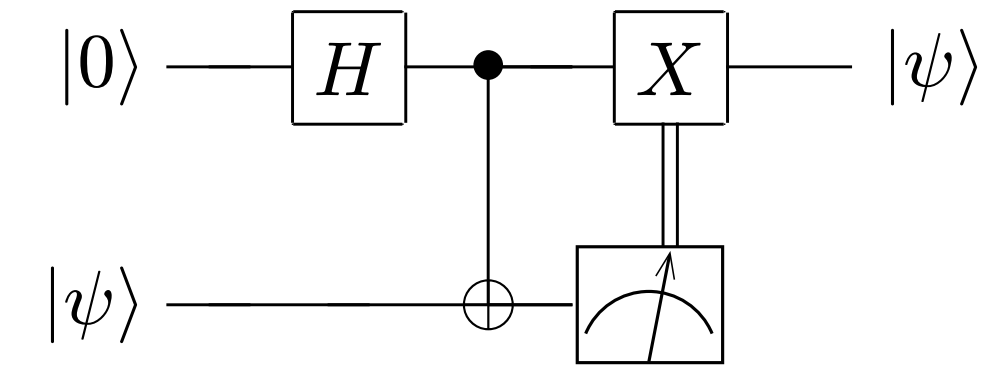
\includegraphics[width=0.4\textwidth]{Figures/1-bit-Teleport.png}
\caption{Circuit for `1-bit teleportation', taken from~\cite{Zhou2000}.}
\label{fig:MSI}
\end{wrapfigure}
A fault tolerant T gate can be realised using a `1-bit teleportation' or state-injection circuit, developed by Chuang et al~\cite{Zhou2000}. This simplified teleportation circuit made up of an ancillae qubit $H\ket{0}=\ket{+}$, Clifford gates, and an additional measurement-controlled correction.\\
By using an appropriately prepared ancilla, this circuit can be used to realise the state $U\ket{\psi}$. To find the required state, we need to commute the operator $U$ through the circuit, which can be done for any diagonal unitary $U\in\mathcal{C}_{n}\forall n\geq 3$~\cite{Zhou2000}. This has the affect of changing the required correction operation $X\rightarrow UXU^{\dagger}$, and changing the ancilla $\ket{+}\rightarrow U\ket{+}$~\cite{Zhou2000}.\\
For the T gate, which satisfies the diagonal requirement, this requires preparing an ancilla $\ket{A}=\ket{0}+\mathe^{i\frac{\pi}{4}}\ket{1}$. Because the state injection circuit is built out of Clifford gates and measurements, the problem of a fault tolerant implementation then reduces to preparing these ancilla states.
\par
A scheme for preparing these ancillae was proposed by Bravyi \& Kitaev, allowing an arbitrarily pure state to be prepared from multiple, imperfectly prepared copies~\cite{Bravyi2005}. This method can be used to prepare $\ket{H}=\cos(\frac{\pi}{8})\ket{0}+\sin(\frac{\pi}{8})\ket{1}$, and a family of other states that are equivalent to $\ket{A}$ up to a Clifford group operation~\cite{Bravyi2005}.\\
Because they can boost a stabilizer code to universality, these states are dubbed `magic states'~\cite{Bravyi2005}. Bravyi \& Kitaev also derived a threshold fidelity for the initial noisy magic states, for the distillation procedure to be able succeed, which corresponds to the edges of an octahedron in the Bloch Sphere defined by the single qubit stabilizer states~\cite{Bravyi2005}. $\ket{A}$ and other T-gate magic states are pure states that project out from the edges of the octahedron, which is shown in Fig.~\ref{fig:octahedron}.\\
An alternative type of magic state, which we will dub $\ket{F}$ for `face'-state, lies at the centre of the faces of this octahedron. This is also shown in Fig.~\ref{fig:octahedron}. However, because there is currently no known deterministic procedure for using face-type states in state injection, fault tolerant computing schemes focus on using circuits built out of Clifford gates and T gates.
\begin{figure}[h]
    \centering
    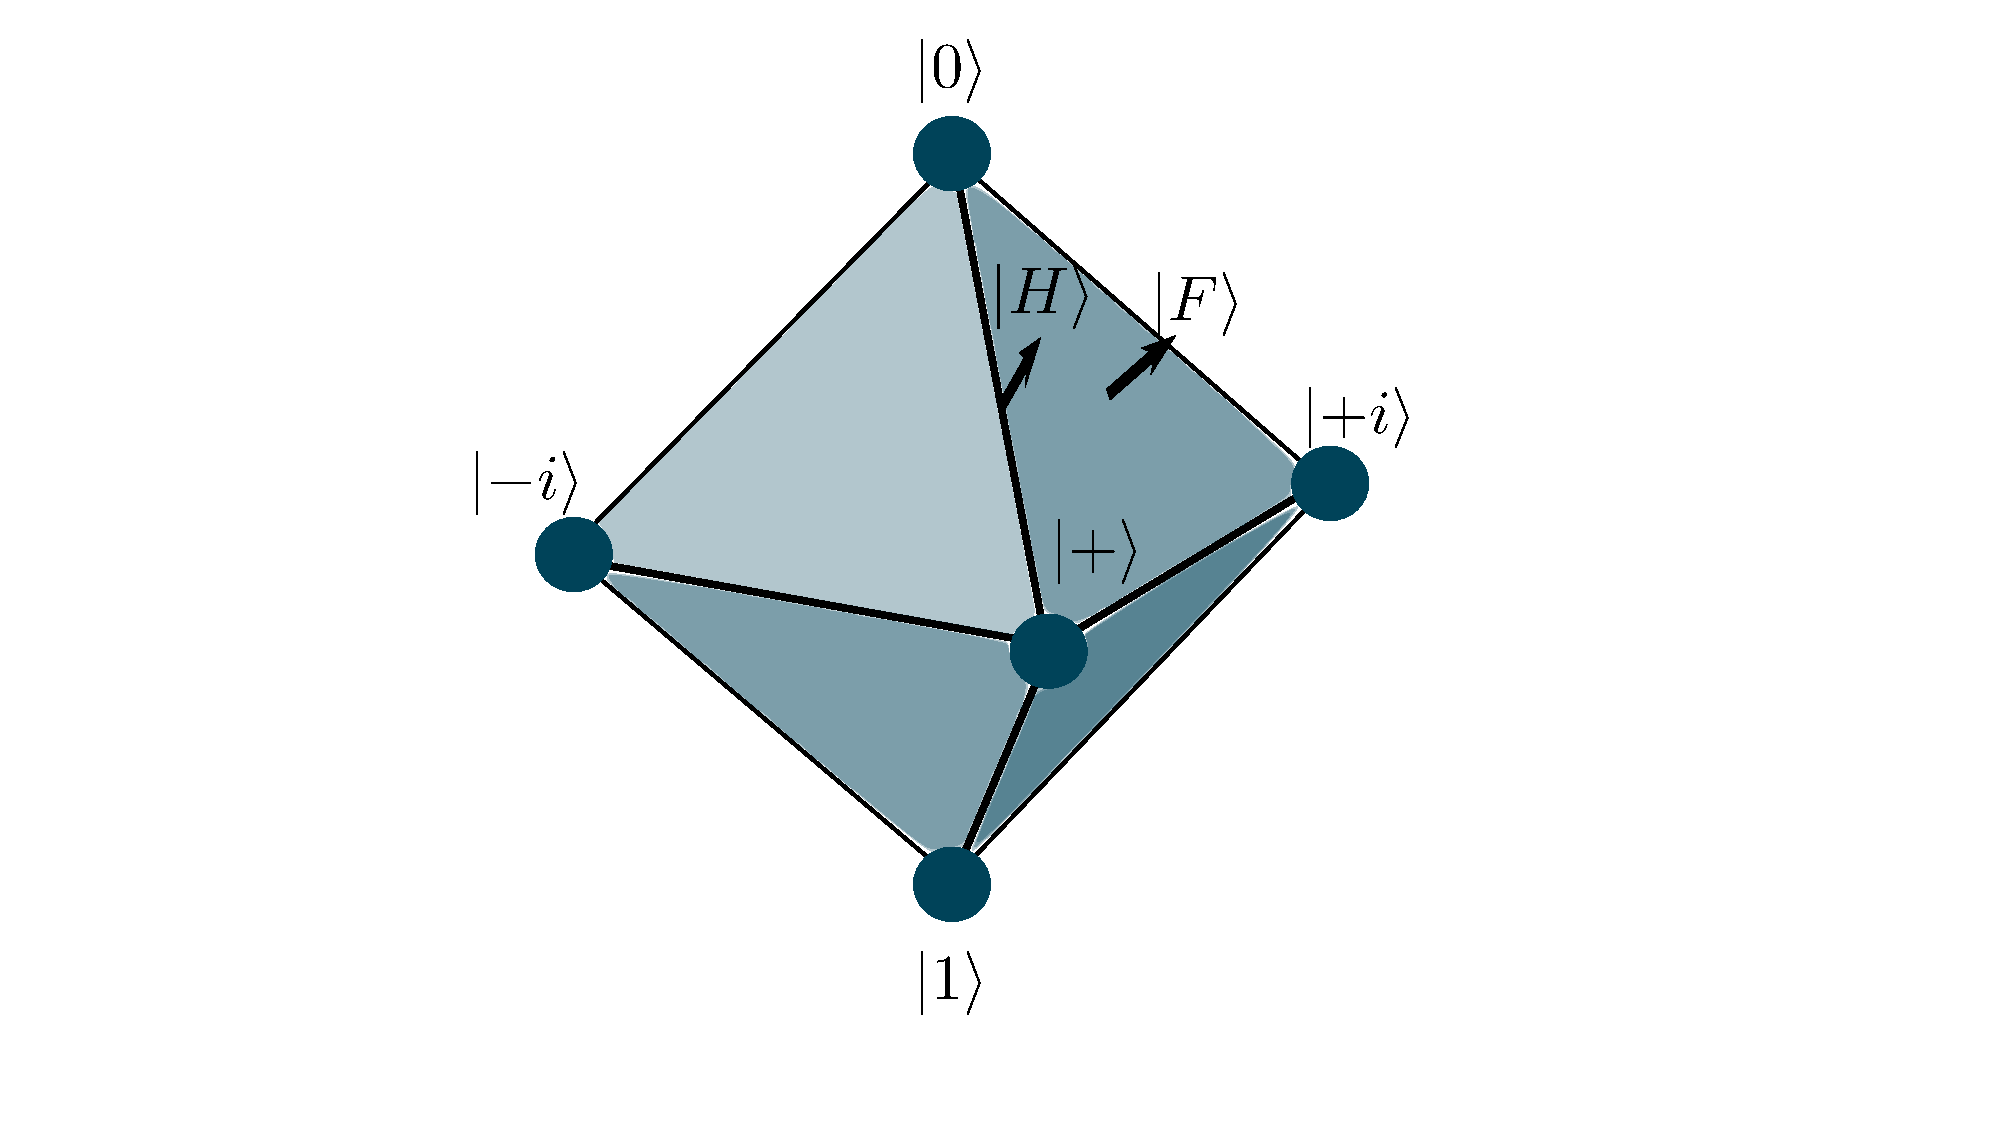
\includegraphics[width=0.75\textwidth]{Figures/octahedron.pdf}
\caption{Representation of the set of classically simulable states in the Bloch Sphere, showing the edge and face-type magic states.}
\label{fig:octahedron}
\end{figure}

\subsubsection{Simulating Clifford+T Circuits}\label{sec:CHP}
The octahedron shown in Fig.~\ref{fig:octahedron} corresponds to convex mixtures of stabilizer states, and as such it also defines the set of efficiently simulable single-qubit states~\cite{Howard2014}. The single qubit Clifford group operations correspond to symmetric rotations of the octahedron, which illustrates the classical simulability of Clifford circuits on stabilizer states. 
\par
An efficient algorithm for classically simulating these Clifford circuits, called `CHP'\footnote{Named for the generators of the n-qubit Clifford group: CNOT, Hadamard and Phase}, was developed by Aaronson \& Gottesman. Using the fact that the Pauli group can be generated by $\pm\mathi, X$ and $Z$, and that stabilizer generators must must have real-valued phase as the group cannot contain the element $-\mathbb{I}$, they represent each stabilizer on $n$ qubits as a $2n+1$ bit binary string. Pairs of the first $2n$ bits describe the Pauli operator on each of the $n$ qubits: \texttt{00} corresponds to $\mathbb{I}$, \texttt{01} to $Z$, \texttt{10} to $X$ and $\texttt{11}$ to $Y$. The final bit $r$ gives the phase of $-1^{r}$.\\
These $n$ stabilizer bit strings are stored in a $2n\times(2n+1)$ tableau. The other $n$ rows are the `destabilizers', a dual set of operators that, together with the stabilizers, generate the full $n$-qubit Pauli group. The \texttt{CHP} method is then capable simulating arbitrary Clifford group operations and Pauli measurements on $n$ qubits in a time $\order{n^{3}}$, by updating the tableau appropriately.
\par
In the paper, Aaronson \& Gottesman also discuss extensions of the CHP method to the case where a quantum computer is furnished with $b$ non-stabilizer ancillae, $d$ of which are subject to Pauli measurements. In this case, the \texttt{CHP} method acquires an exponential scaling $\order{2^{2b+2d}}$~\cite{Aaronson2004a}. As a Clifford+T computing scheme would consume all magic states, this  implies $b=d\equiv t$, giving an effective scaling of $\order{2^{4t}}$, where $t$ is the total `$t$ count' of the circuit~\cite{Aaronson2004a,Bravyi2015}. Interestingly, this method performs lightly better if the formalism is adapted to describe non-Clifford gates, giving a scaling $\order{4^{bd}}$ for $b$ gates acting on at most $d$ qubits. In the case of $t$ T-gates acting on single qubits, we obtain a scaling $\order{4^{t}}$~\cite{Aaronson2004a}.
\par
This exponential dependence on the T-count is expected; adding appropriate non-Clifford gates (either directly or with ancillae) promotes our quantum computation to universality, and thus it should no-longer be classically simulable.

\subsubsection{Contextuality}\label{sec:context}
Most recently, a property of quantum mechanics called contextuality has emerged as an alternative requirement for quantum advantage. Contextuality in fact seems to correspond to a property, $\text{prop}\left(\mathcal{D}\right)$, required for quantum speedup in the `Clifford+T' picture of quantum computing.
\par
Contextuality is understood as a generalisation of non-locality, which derives from a theorem by Bell, Kochen \& Specker demonstrating that a measurement outcome in quantum mechanics cannot be understood as revealing a `hidden variable' that describes the state of the system~\cite{Howard2014}. What makes this interesting as a candidate for quantum advantage is that it is a feature that cannot be replicated in classical models. For example, Spekken's toy model, an classical model with an `epistemic' restriction preventing any more than half of the `hidden variables' being known, is capable of describing other `quantum' features like entanglement, but cannot demonstrate contextuality~\cite{Spekkens2007}. 
\par
It has been demonstrated that the onset of contextuality for qudits, $d$-dimensional elements where $d>2$, corresponds exactly with leaving the set of efficiently simulable states. For qudits, this set is slightly larger than the set of stabilizer states, but any state outside this set is sufficient to promote a Clifford circuit to universality~\cite{Howard2014}.\\
However, for qubits, the case is slightly more complicated. The set of simulable states in this case coincides exactly with the set of stabilizer states, but it has in fact been shown that qubits demonstrate `state-independent' contextuality: even stabilizer states will violate `contextuality' inequalities~\cite{Howard2014}. However, it has nonetheless been shown that magic states give larger violations of contextuality inequalities than arbitrary quantum states, and that this is largest for the face-type states $\ket{F}$~\cite{Howard2014}.

\ifstandalone 
\bibliography{../MResProject.bib,../ManualEntries.bib}
\fi
\end{document}
